\documentclass[11pt, oneside, a4paper, titlepage]{article}
\usepackage[most]{tcolorbox}
\usepackage{geometry}
\geometry{a4paper, left=0.1cm, right=0.1cm,top=1cm,bottom=0.1cm}
\definecolor{titleBack}{RGB}{0,66,21}
\title{CV}
\begin{document}
	\begin{tcolorbox}
		\tcbset{colframe=gray!25,colback=titleBack, arc=0mm}
		\begin{minipage}{4.5cm}
			\hspace*{0.5cm}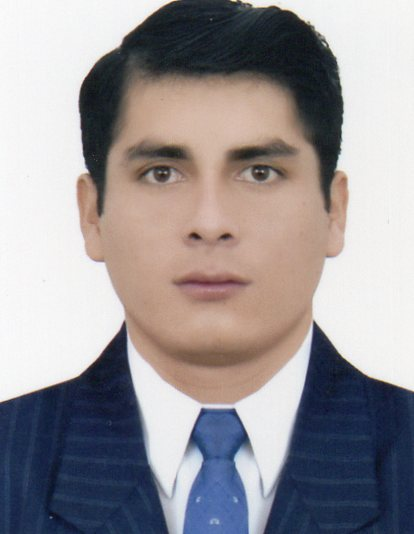
\includegraphics[width=2cm]{img004}
		\end{minipage}
		\begin{minipage}{15cm}
			\begin{center}
				\Huge{\textcolor{black}{\textbf{Alex Vargas Galvez}}}\\
				\vspace{0.5cm}
				\Large{\textcolor{black}{Egresado de redes y telecomunicaciones, estudiante de informática}}
			\end{center}			
		\end{minipage}
	\end{tcolorbox}
	
	\tcbset{colframe=white, colback=white, arc=8mm}
	\begin{tcolorbox}
		\begin{minipage}[t]{8cm}
			\vspace{-0.5cm}
			\begin{tcolorbox}[grow to left by=0.6cm, colback=gray!15, colframe=white]
				\section*{Contacto}
				\begin{tabular}{r l}
					Cel: & +51 973402483 \\
					Email: & alex.vargas.galvez.98@gamail.com\\
					Linkedin: & @alexvargas\\
					Github: & alexvargasdev 
				\end{tabular}
				\\
				\section*{Perfil}
				En cada etapa de mi formación he logrado desarrollar mis habilidades tanto profesionales como sociales mejorando así mi liderazgo, adaptabilidad a múltiples circunstancias y valorar mucho el trabajar en equipo. El aspecto laboral es una de mis pasiones, por ello siempre doy lo mejor de mí, para ello me encuentro en constante búsqueda de adquirir conocimientos y estrategias adecuadas para utilizarlas a nivel profesional y personal.
				
				\section*{Habilidades}
				
				\begin{itemize}
					\item Liderazgo
					\item Pro-actividad
					\item Adaptabilidad
					\item Perseverancia
				\end{itemize}
				
				\section*{Conocimiento de Software}
				
				\begin{itemize}
					\item Python
					\item Java
					\item Matlab
					\item Java Scrip
					\item Node JS
					\item R 
					\item Microsoft Office
					
				\end{itemize}
				
				\section*{Idiomas}
				
				\begin{itemize}
					\item Español
					\item Quechua
					\item Ingles (Intermedio)
				\end{itemize}
			\end{tcolorbox}
		\end{minipage}
		\begin{minipage}[t]{11cm}
			\vspace{-0.5cm}
			\begin{tcolorbox}[grow to right by=0.75cm, colframe=white, colback=white]
				\section*{Educación}
				\begin{itemize}
					\item \textbf{\textsc{Instituto Tecnológico IDAT}}\\
					\emph{Sistemas de telecomunicaciones}\\
					\emph{\textbf{Mayo 2015 - diciembre 2018}}
					\item \textbf{\textsc{Universidad Nacional San Cristóbal de Huamanga}}\\
					\emph{Ingeniería de sistemas}\\
					\emph{\textbf{Cursando}}
				\end{itemize}
				\section*{Cursos y talleres}
				\begin{itemize}
					\item Internet de las cosas\\
					\emph{\textbf{CISCO}}
					\item Introducción a ciberseguridad \\
					\emph{\textbf{CISCO}}
					\item Malware en dispositivos \\
					\emph{\textbf{ESET}}
					\item Desafíos de la red Wi-Fi corporativa,solución Wi-Fi Enterprise TP-LINK y UBIQUITI\\
					\emph{\textbf{Instituto SISE - TP-LINK - UBIQUITI}}
				\end{itemize}
				\section*{Experiencia laboral}
				\begin{itemize}
					\item Corte Suprema de Justicia de Lima\\
					\emph{\textbf{Asistente de Soporte Técnico en el área de Informática}}\\
					\emph{Enero 2017 - enero 2018}\\
					{Trabajos realizados:}
					\begin{itemize}
						\item Soporte de redes LAN y WAN.
						\item Conexiones de radio enlace.
						\item Segmentación de VLANS.
						\item Configuraciones de routes, switchs, anexos, impresoras en red y puntos de acceso Wi-Fi o físico.
						\item Formateo de computadoras. 
						\item Clonación de discos duros
						\item Reparación de caja del CPU.
						\item Atención informática a usuarios.
						\item Instalación de softwares.
						\item Inventario físico de computadoras y otros asignados por el área.
						
					\end{itemize}
				\end{itemize}
			\end{tcolorbox}
		\end{minipage}
	\end{tcolorbox}
	
\end{document}